\documentclass{beamer}

% does not look nice, try deleting the line with the fontenc.
\usepackage[english]{babel}
\usepackage{amsmath}
\usepackage[latin1]{inputenc}
\usepackage{units}
\usepackage{colortbl}
\usepackage{multimedia}
\usepackage{bm}

\mode<presentation>
{
  \usetheme{Boadilla}
  \useoutertheme{infolines}
  \setbeamercovered{transparent} 
}
	

\title[Bayesian Optimization Overview]{\textsc{Bayesian Optimization Overview}}

%\subtitle{Industrial-scale experimental results\\} % (optional)

\author[]{Marco Forgione}

\institute[IDSIA]{
	\inst{1}IDSIA Dalle Molle Institute for Artificial Intelligence SUPSI-USI, Lugano, Switzerland} 


\date[]{\today}


\subject{Bayesian Optimization}


%% MATH DEFINITIONS %%
%\newcommand{\R}{\mathcal{R}}
%\newcommand{\du}{\delta u}
%\newcommand{\dy}{\delta y}
%\newcommand{\DU}{\Delta U}
%\newcommand{\DY}{\Delta Y}
%\newcommand{\abs}[1]{\left | #1 \right |}
\newcommand{\norm}[1]{\left \lVert #1 \right \rVert}
%\newcommand{\relphantom}[1]{\mathrel{\phantom{#1}}}
%\newenvironment{matrixc}{\begin{array}{c}\left[}{\end{array}\right]}
\DeclareMathOperator*\argmin{arg \, min}
%\DeclareMathOperator*\argmax{arg \, max}
%\DeclareMathOperator*\fit{fit}
%\DeclareMathOperator*\RMSE{RMSE}
%\DeclareMathOperator*\diag{diag}
%\DeclareMathOperator*\diet{diet}
%\DeclareMathOperator*\Risk{Risk}
%\DeclareMathOperator*\Num{Num}
%\DeclareMathOperator*\Den{Den}
%\DeclareMathOperator*\Rat{Rat}
\DeclareMathOperator*\cov{cov}
%\DeclareMathOperator*\Var{Var}
%\DeclareMathOperator*\SSR{SSR}
%\setcounter{MaxMatrixCols}{20}
%\newcommand{\pdiff}[2]{\frac{\partial #1}{\partial #2}}
%\definecolor{mypink1}{rgb}{0.858, 0.188, 0.478}
%\definecolor{olive}{RGB}{85, 107, 47}
\definecolor{orange}{RGB}{204, 85, 0}

%\definecolor{mypink3}{cmyk}{0, 0.7808, 0.4429, 0.1412}
%\definecolor{mygray}{gray}{0.6}
%\definecolor{olivegreen}[RGB]{85, 107, 47}

\newcommand{\K}{K}
\newcommand{\M}{M}
\newcommand{\Mo}{M_o}
\newcommand{\So}{S_o}
\newcommand{\Smod}{S}
\newcommand{\parcolor}[1]{{\color{orange}#1}}

\definecolor{darkgreen}{RGB}{20,150,50}

\begin{document}

\begin{frame}
  \titlepage
\end{frame}

%\begin{frame}
%\frametitle{Outline}
%\tableofcontents
%\end{frame}
\begin{frame}{Motivations}
Obtaining the \structure{predictive model} for {MPC} is \alert{costly} and \alert{time-consuming}.
\vskip 1em
Typically, models are obtained through Physical modeling or Identification
\begin{itemize}
 \item Requires \structure{domain knowledge} and/or \structure{ad-hoc identification experiments}
 \item A trade-off emerges between accuracy and complexity
\end{itemize}
\vskip 1em
It is often difficult to decide \emph{a priori} how accurate the predictive model should be in order to achieve satisfactory closed-loop performance.
\vskip 1em
\pause
In this work:
\begin{itemize}
\item We introduce a \structure{data-driven framework} aimed at finding the best model for MPC \structure{from calibration experiments}
\pause
\item We specialize this framework for a \structure{hierarchical MPC} architecture often encountered in industrial applications
\end{itemize}
\end{frame}


\begin{frame}{Bayesian Optimization}{Overview}
One of the best \emph{off-the-shelf} global optimization algorithms% to date
\begin{itemize}
 \item Iteratively updates a \structure{stochastic surrogate model} of the unknown $J(\theta)$ via Bayesian inference. Typically, a Gaussian Process (GP)
 \item Balances \structure{exploitation} and \structure{exploration} by optimizing an 
 \structure{acquisition function} $A(\theta)$ instead of the surrogate model directly
 \item The acquisition function $A(\theta)$ favors points with estimated \structure{good performance} 
 $\rightarrow$ exploitation and/or \structure{high variance} $\rightarrow$ exploration
 \item The acquisition function $A(\theta)$ is (relatively) cheap to evaluate. It is a mathematical object!
\end{itemize}
\pause
%\vskip 1em
%Steps of BO: for $i=1,2,\dots i_{\rm max}$
%\begin{enumerate}
% \item \textbf{Execute} experiment with $\theta_i$, measure $J_i = J(\theta_i) + e_i$
% \item \textbf{Refine} the stochastic GP model $\theta \rightarrow J(\theta)$ 
% \item \textbf{Construct} acquisition function $A(\theta)$
% \item \textbf{Maximize} $A(\theta)$ to obtain next query point $\theta_{i+1}$
%\end{enumerate}
\end{frame}

\begin{frame}{Bayesian Optimization}{Gaussian Process}
\begin{itemize}
\item The function $J(\theta)$ assumed Gaussian with \structure{prior} mean $E[J(\theta)] = \mu(\theta)$ and 
 covariance $\cov[J(\theta_1), J(\theta_2)] = \kappa(\theta_1, \theta_2)$.
\item The \structure{posterior} mean and covariance given a new observation $(\theta_i, J_i)$ is obtained in closed form
\end{itemize}

\only<1>{
\centering 
0 points
\vskip -1em
\begin{figure}
    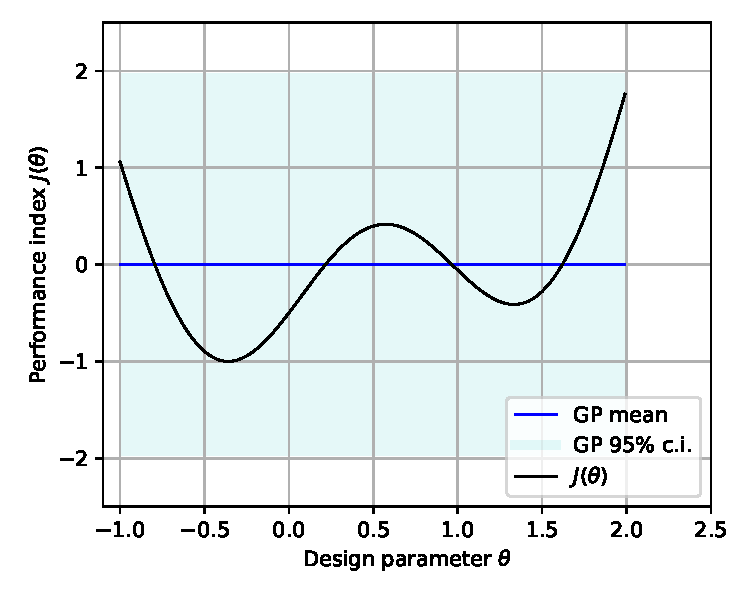
\includegraphics[width=.5\textwidth]{img/GP_fit/GP_fit_0.pdf}
\end{figure}
}
\only<2>{
\centering 
1 point
\vskip -1em
\begin{figure}
    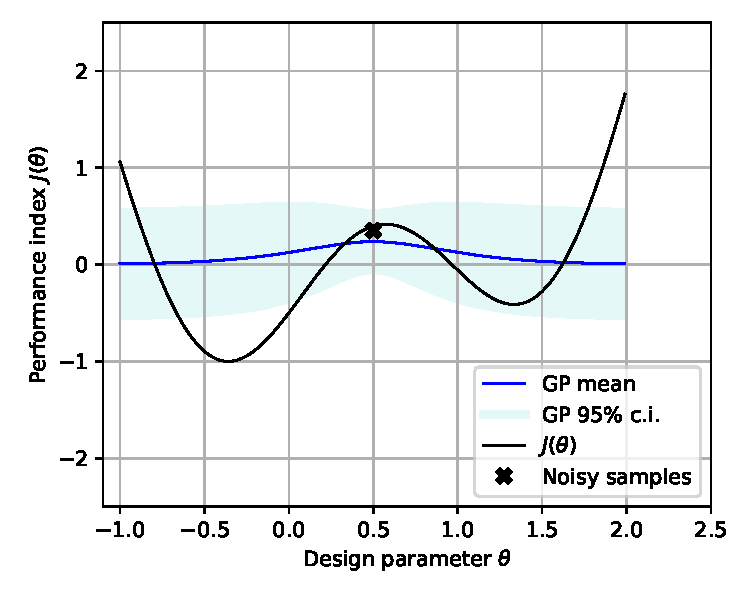
\includegraphics[width=.5\textwidth]{img/GP_fit/GP_fit_1.pdf}
\end{figure}
}
\only<3>{
\centering 
2 points
\vskip -1em
\begin{figure}
    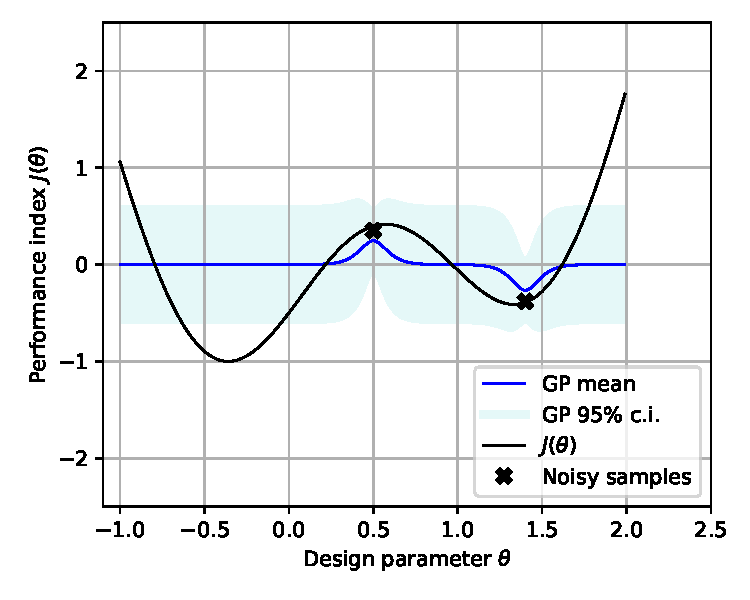
\includegraphics[width=.5\textwidth]{img/GP_fit/GP_fit_2.pdf}
\end{figure}
}
\only<4>{
\centering 
4 points
\vskip -1em
\begin{figure}
    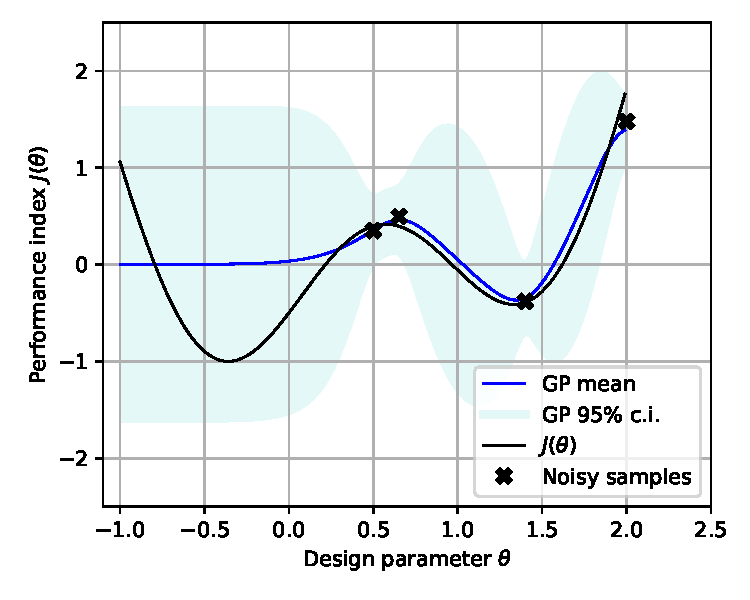
\includegraphics[width=.5\textwidth]{img/GP_fit/GP_fit_4.pdf}
\end{figure}
}
\only<5>{
\centering 
6 points
\vskip -1em
\begin{figure}
    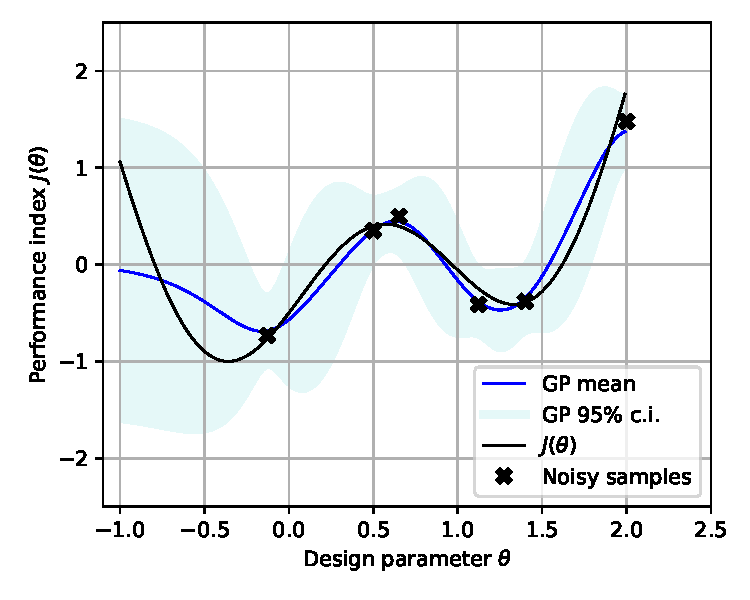
\includegraphics[width=.5\textwidth]{img/GP_fit/GP_fit_6.pdf}
\end{figure}
}
\only<6>{
\centering 
20 points
\vskip -1em
\begin{figure}
    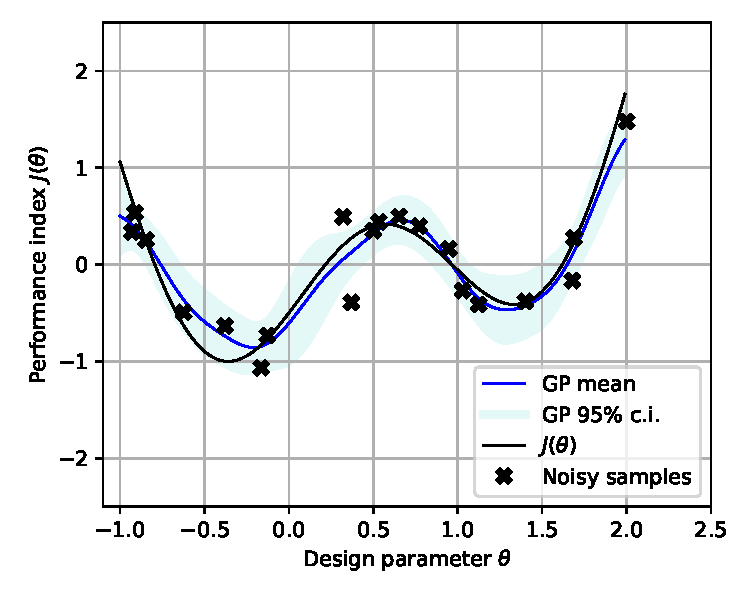
\includegraphics[width=.5\textwidth]{img/GP_fit/GP_fit_20.pdf}
\end{figure}
}

\end{frame}

\begin{frame}{Bayesian Optimization}{Acquisition function}
The GP provides the \structure{probability distribution} of $J(\theta)$ for each parameter $\theta$.\\
This probability is used to define an \structure{acquisition function}, \emph{e.g.},
\vskip 1em
\begin{columns}
\column{.5 \textwidth}
\centering
Probability of Improvement
$$A(\theta)  = \mathrm{PI}(\theta)= p(J(\theta) \leq J^{\mathrm{min}})$$
\column{.5 \textwidth}
\centering
Expected improvement
$$A(\theta)\!=\!\mathrm{EI}(\theta)\!=\!\mathbb{E}[\max\left(0, J^{\mathrm{min}}\!-\!J(\theta)\right)] $$
\end{columns}
\begin{figure}
    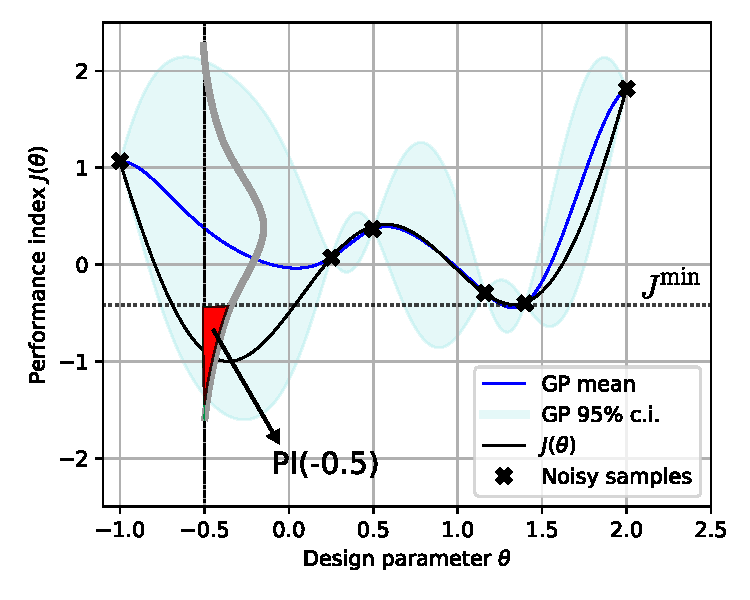
\includegraphics[width=.5\textwidth]{img/PI_fit_6.pdf}
\end{figure}
\end{frame}

\begin{frame}{Bayesian Optimization}{Overview}
Steps of BO: for $i=1,2,\dots i_{\rm max}$
\begin{enumerate}
 \item \textbf{Execute} experiment with $\theta_i$, measure $J_i = J(\theta_i) + e_i$
 \item \textbf{Update} the GP model $\theta \rightarrow J(\theta)$ with $(\theta_i, J_i)$
 \item \textbf{Construct} acquisition function $A(\theta)$
 \item \textbf{Maximize} $A(\theta)$ to obtain next query point $\theta_{i+1}$
\end{enumerate}
\vskip -1em
\begin{columns}
 \column{.5\textwidth}
 \begin{figure}
    GP at iteration $i$
    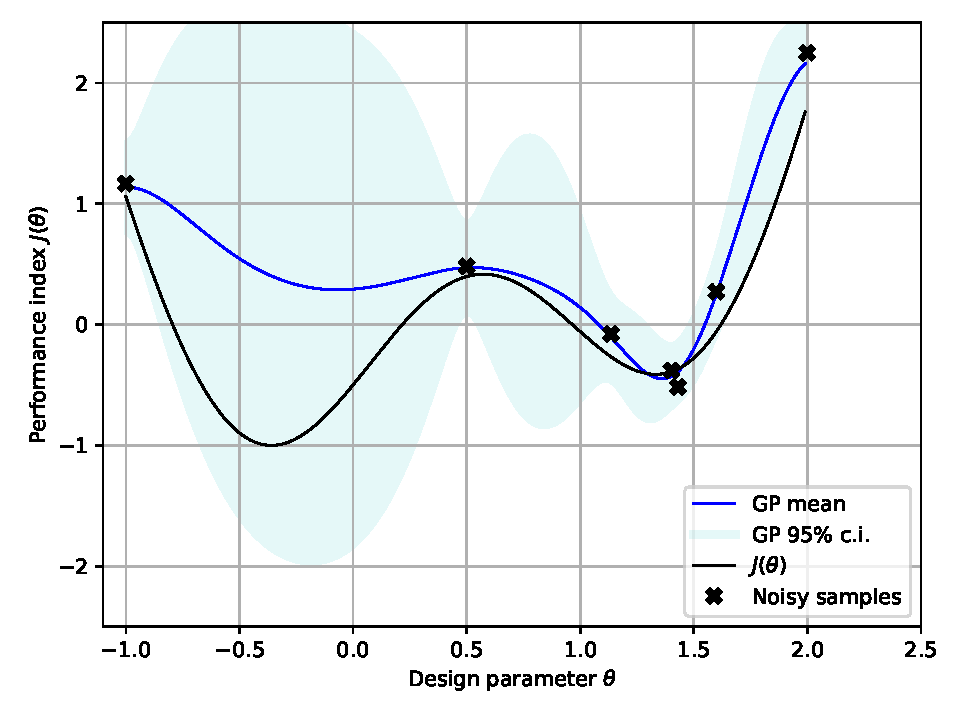
\includegraphics[width=.9\textwidth]{img/BO/BO_fit_4.pdf}
\end{figure}
 \column{.5\textwidth}
\begin{figure}
$A(\theta)$ at iteration $i$
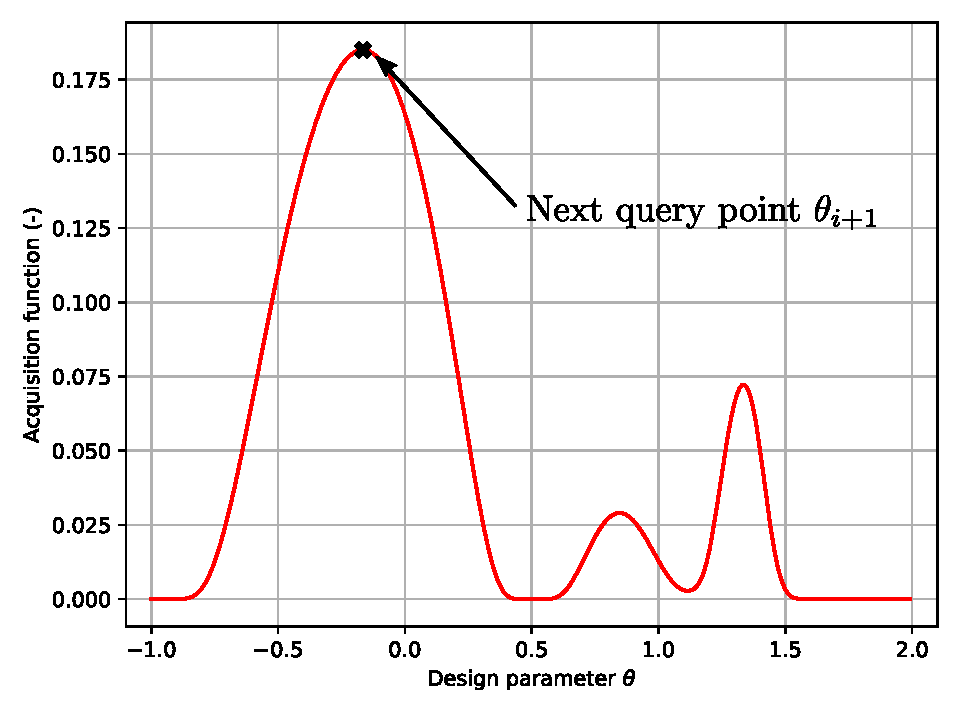
\includegraphics[width=.9\textwidth]{img/BO/BO_acq_4_annot.pdf}
\end{figure}
\end{columns}
%\pause
%Actually, first $n_{\rm init}$ samples usually chosen randomly.
\end{frame}


\begin{frame}{Bayesian Optimization}{Example}
\only<1>{
\centering
iteration 6
}
\only<2>{
\centering
iteration 7
}
\only<3>{
\centering
iteration 8
}
\only<4>{
\centering
iteration 9
}
\only<5>{
\centering
iteration 20
}
\vskip 1 em
\begin{columns}
\column{.5\textwidth}
\only<1>{
\centering 
GP fit
\vskip -.5em
\begin{figure}
    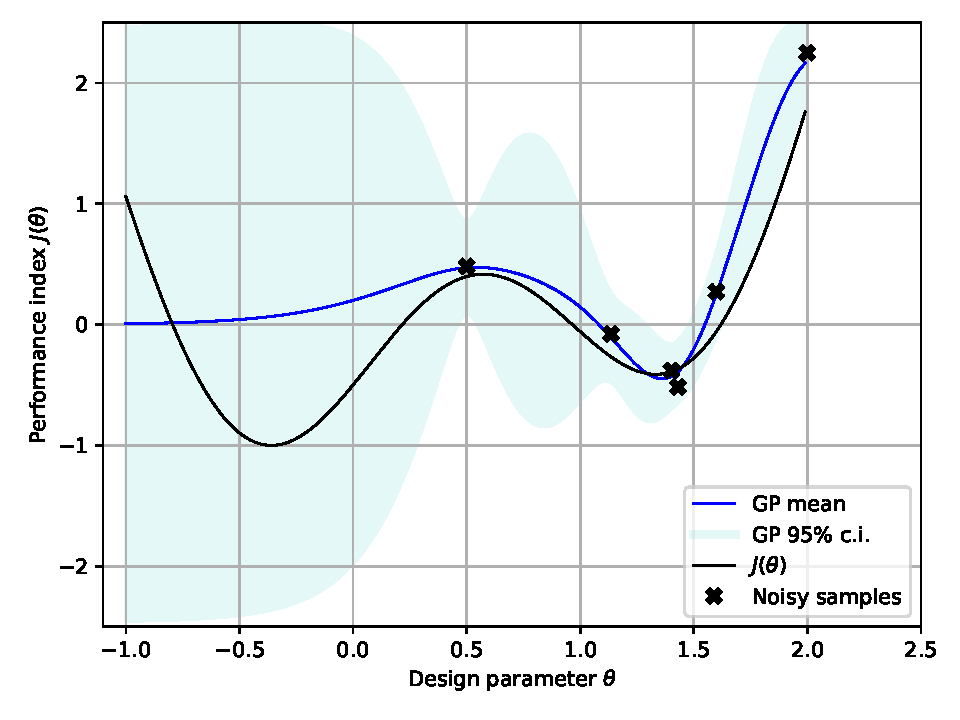
\includegraphics[width=\textwidth]{img/BO/BO_fit_3.pdf}
\end{figure}
}
\only<2>{
\centering 
GP fit
\vskip -.5em
\begin{figure}
    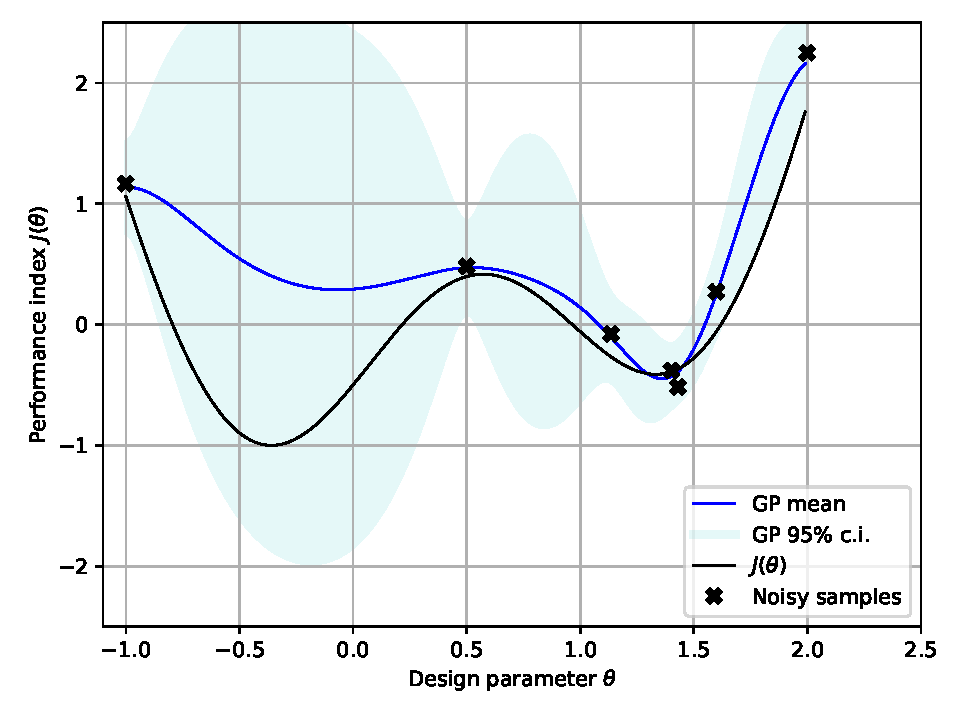
\includegraphics[width=\textwidth]{img/BO/BO_fit_4.pdf}
\end{figure}
}
\only<3>{
\centering 
GP fit
\vskip -.5em
\begin{figure}
    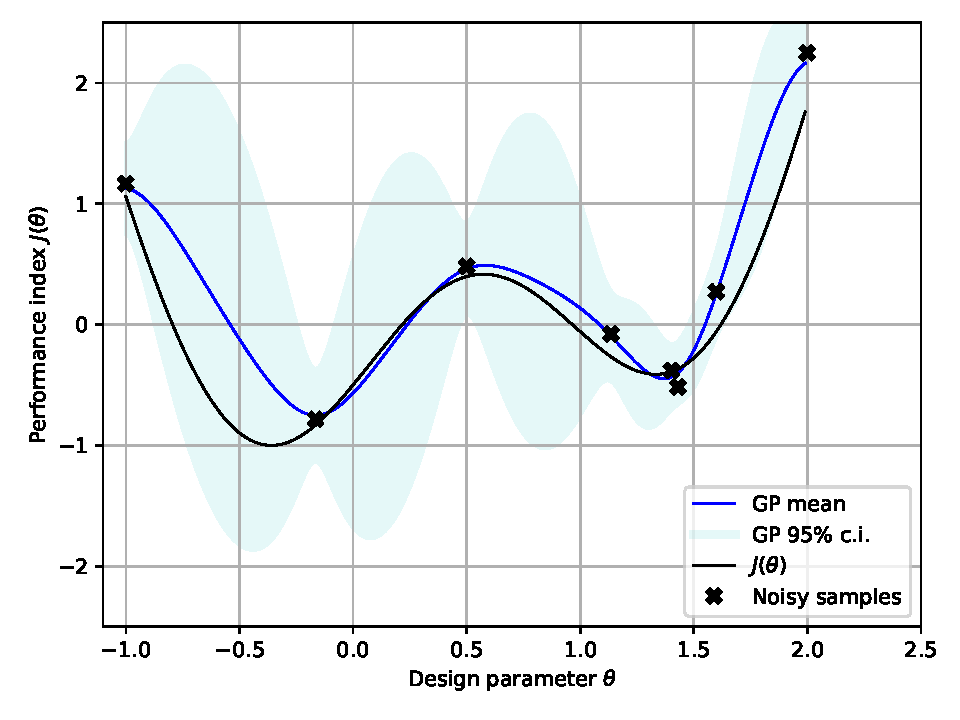
\includegraphics[width=\textwidth]{img/BO/BO_fit_5.pdf}
\end{figure}
}
\only<4>{
\centering 
GP fit
\vskip -.5em
\begin{figure}
    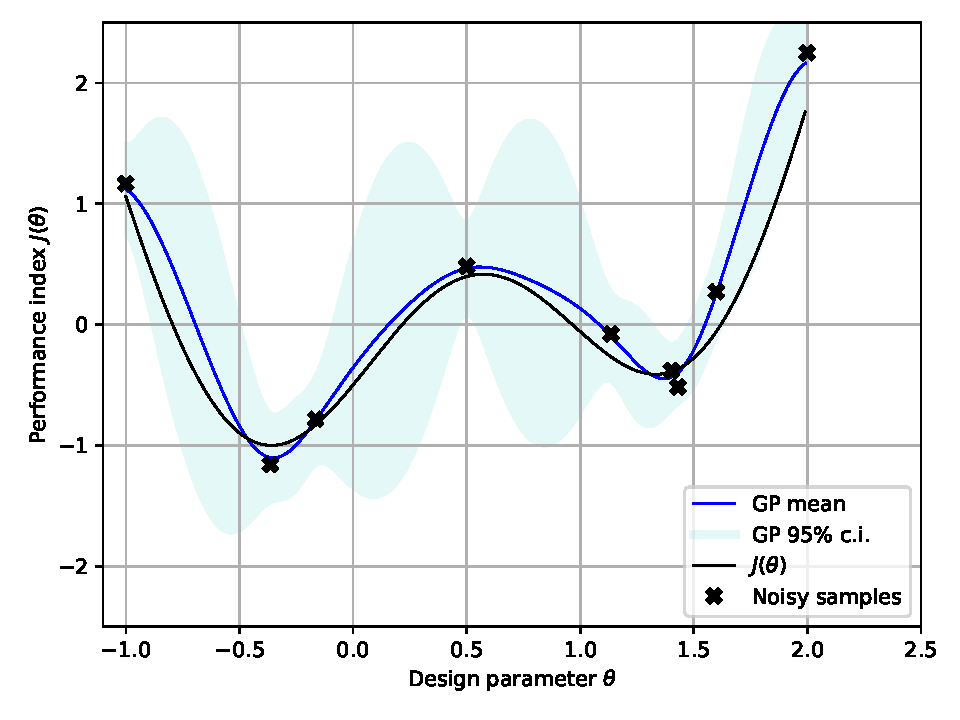
\includegraphics[width=\textwidth]{img/BO/BO_fit_6.pdf}
\end{figure}
}
\only<5>{
\centering 
GP fit
\vskip -.5em
\begin{figure}
    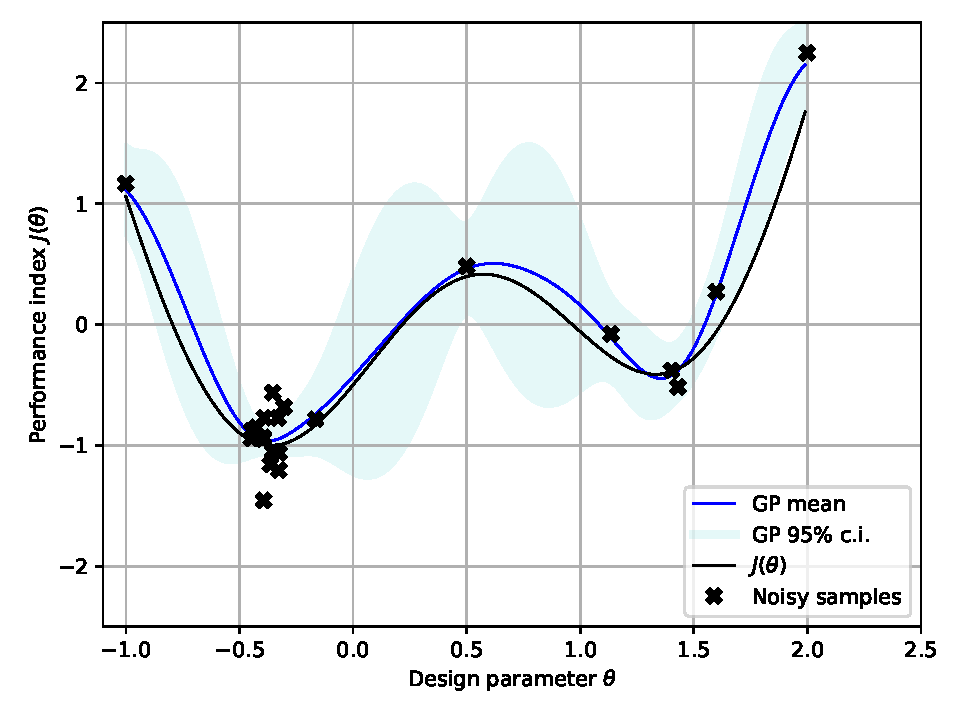
\includegraphics[width=\textwidth]{img/BO/BO_fit_19.pdf}
\end{figure}
}

\column{.5\textwidth}
\only<1>{
\centering 
$A(\theta) = \mathrm{EI}(\theta)$
\vskip -.5em
\begin{figure}
    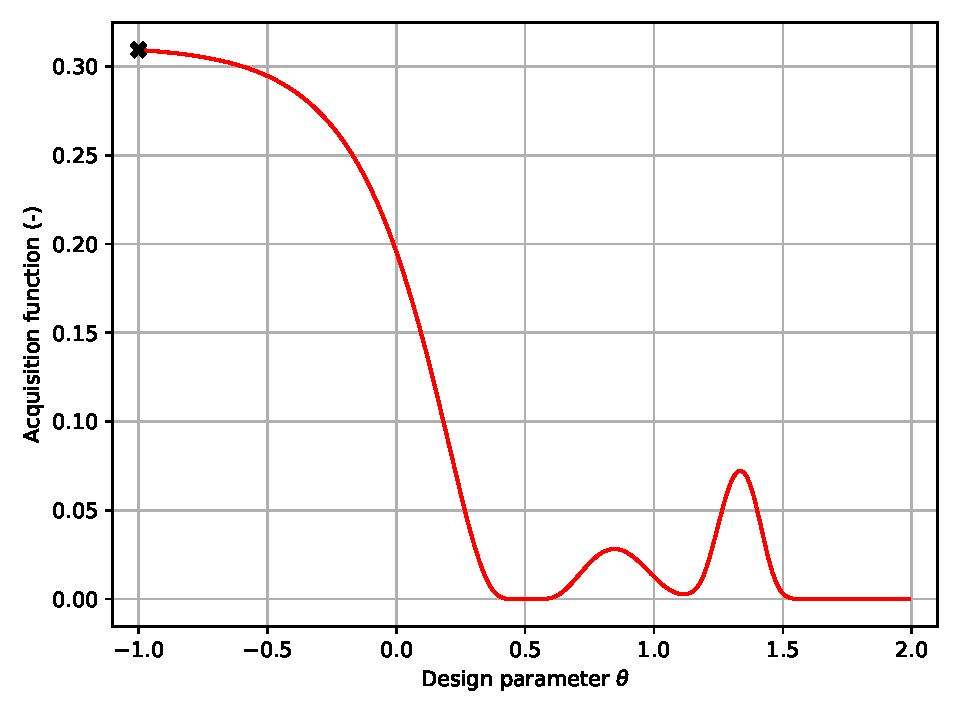
\includegraphics[width=\textwidth]{img/BO/BO_acq_3.pdf}
\end{figure}
}
\only<2>{
\centering 
$A(\theta) = \mathrm{EI}(\theta)$
\vskip -.5em
\begin{figure}
    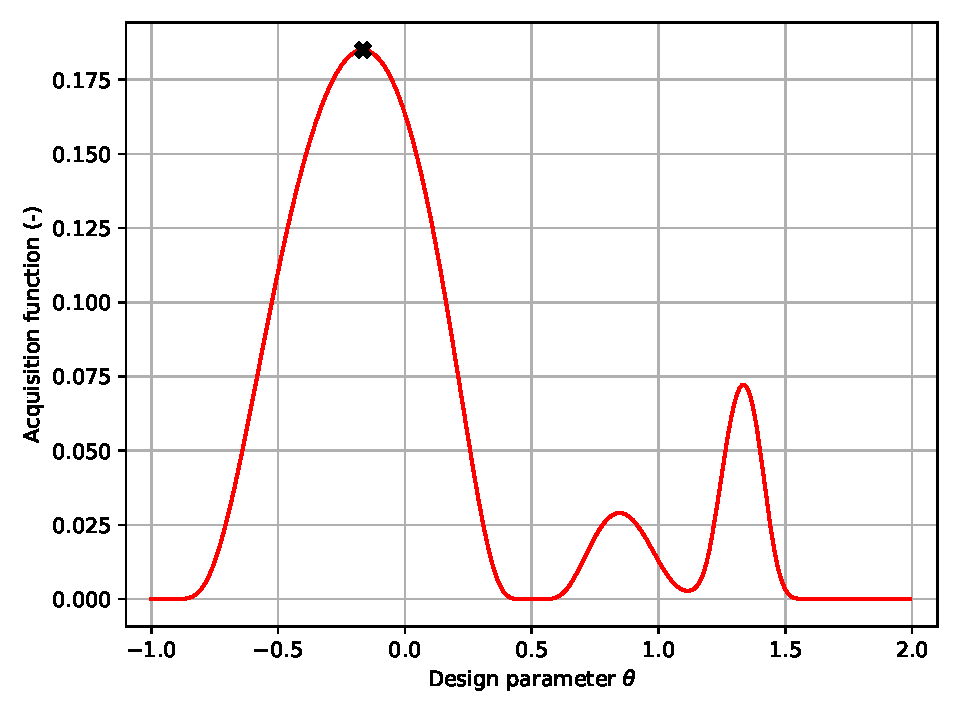
\includegraphics[width=\textwidth]{img/BO/BO_acq_4.pdf}
\end{figure}
}
\only<3>{
\centering 
$A(\theta) = \mathrm{EI}(\theta)$
\vskip -.5em
\begin{figure}
    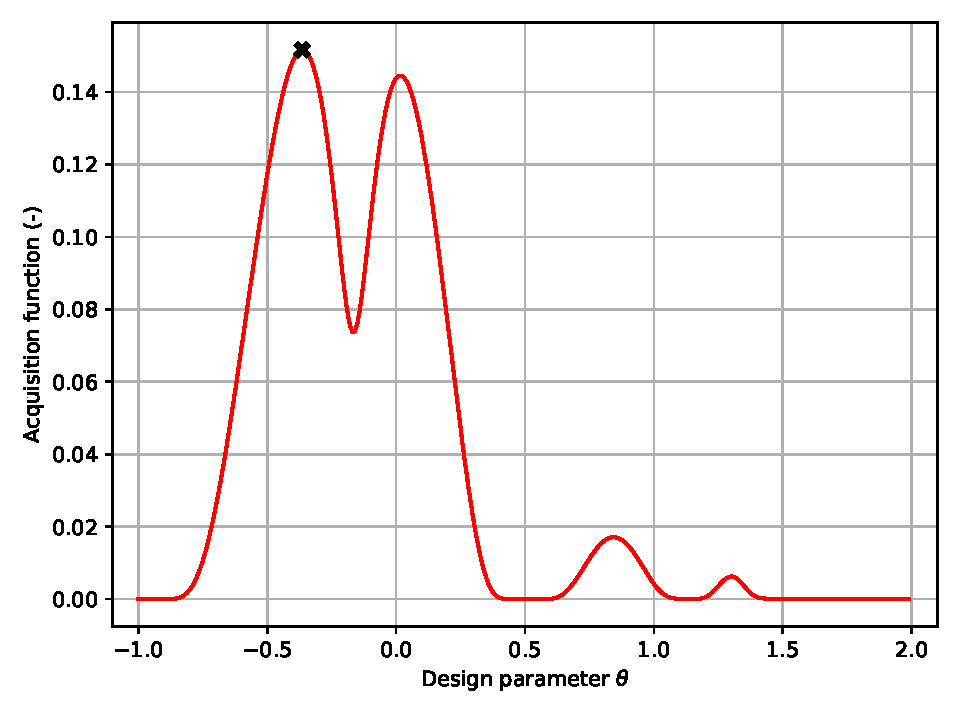
\includegraphics[width=\textwidth]{img/BO/BO_acq_5.pdf}
\end{figure}
}
\only<4>{
\centering 
$A(\theta) = \mathrm{EI}(\theta)$
\vskip -.5em
\begin{figure}
    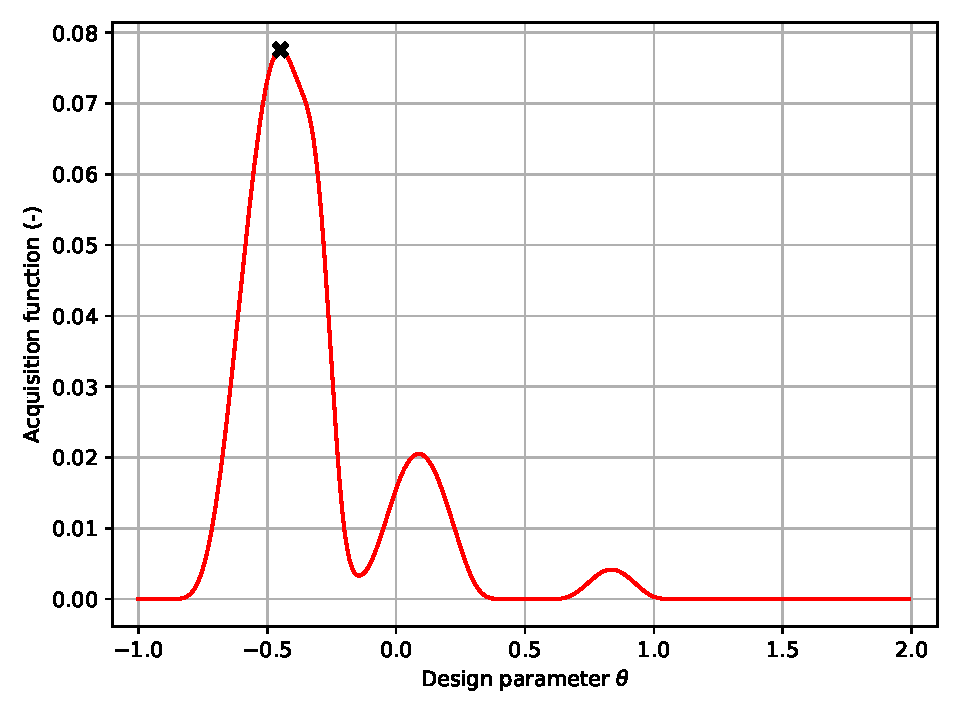
\includegraphics[width=\textwidth]{img/BO/BO_acq_6.pdf}
\end{figure}
}
\only<5>{
\centering 
$A(\theta) = \mathrm{EI}(\theta)$
\vskip -.5em
\begin{figure}
    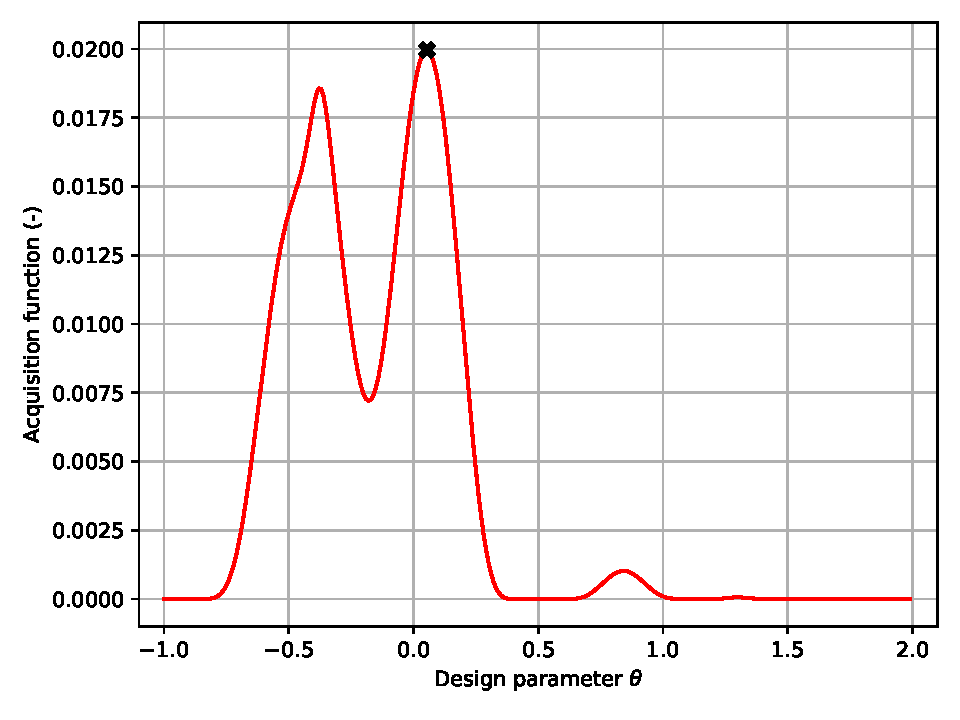
\includegraphics[width=\textwidth]{img/BO/BO_acq_19.pdf}
\end{figure}
}
\end{columns}
\end{frame}

\begin{frame}{Bayesian Optimization}{Example}
\centering
iteration 10
\begin{columns}
\column{.5\textwidth}
   \begin{figure}
   Bayesian Optimization
   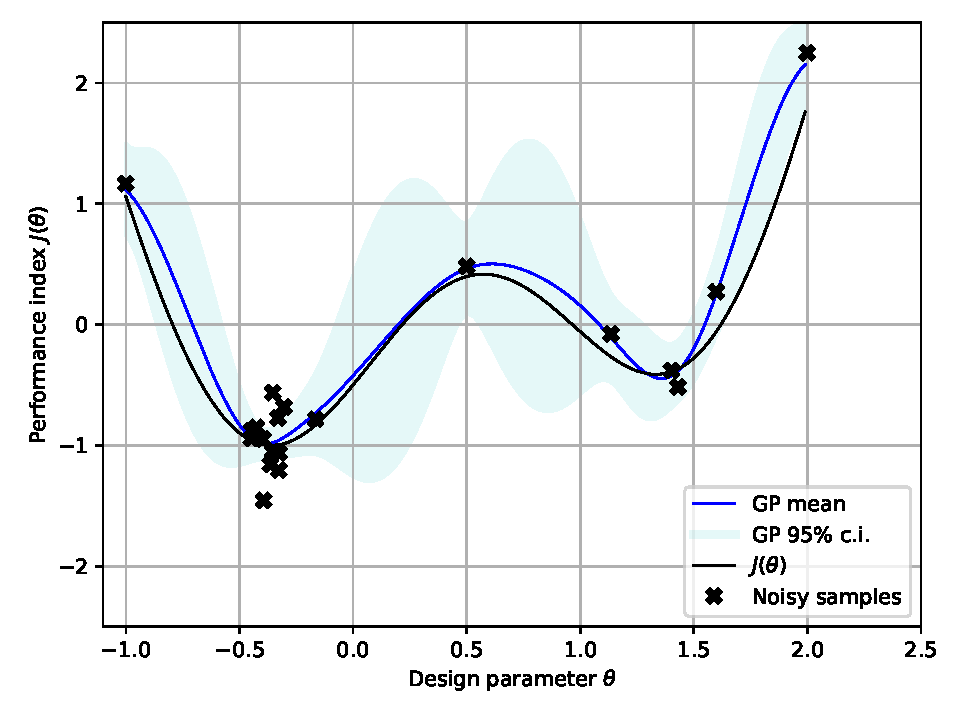
\includegraphics[width=\textwidth]{img/BO/BO_fit_17.pdf}
   \end{figure}  
 \column{.5\textwidth}
   \begin{figure}
 Random sampling
   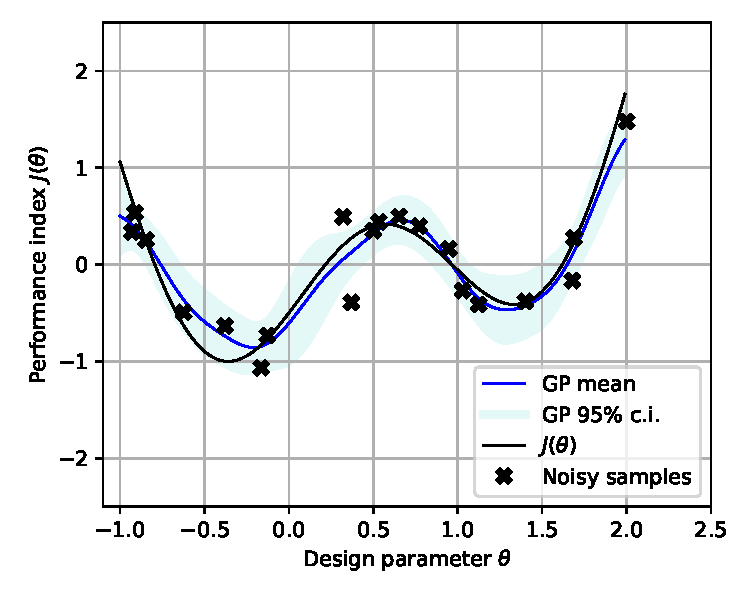
\includegraphics[width=\textwidth]{img/GP_fit/GP_fit_20.pdf}
   \end{figure}  
\end{columns}
\end{frame}


\begin{frame}{}{}
\begin{center}
\huge{\structure{Thank you.\\ Questions?}}
\end{center}
\end{frame}

	
\end{document}
